%%
%% This is file `sample-sigconf-authordraft.tex',
%% generated with the docstrip utility.
%%
%% The original source files were:
%%
%% samples.dtx  (with options: `all,proceedings,bibtex,authordraft')
%%
%% IMPORTANT NOTICE:
%%
%% For the copyright see the source file.
%%
%% Any modified versions of this file must be renamed
%% with new filenames distinct from sample-sigconf-authordraft.tex.
%%
%% For distribution of the original source see the terms
%% for copying and modification in the file samples.dtx.
%%
%% This generated file may be distributed as long as the
%% original source files, as listed above, are part of the
%% same distribution. (The sources need not necessarily be
%% in the same archive or directory.)
%%
%%
%% Commands for TeXCount
%TC:macro \cite [option:text,text]
%TC:macro \citep [option:text,text]
%TC:macro \citet [option:text,text]
%TC:envir table 0 1
%TC:envir table* 0 1
%TC:envir tabular [ignore] word
%TC:envir displaymath 0 word
%TC:envir math 0 word
%TC:envir comment 0 0
%%
%%
%% The first command in your LaTeX source must be the \documentclass
%% command.
%%
%% For submission and review of your manuscript please change the
%% command to \documentclass[manuscript, screen, review]{acmart}.
%%
%% When submitting camera ready or to TAPS, please change the command
%% to \documentclass[sigconf]{acmart} or whichever template is required
%% for your publication.
%%
%%
\documentclass[sigconf,authordraft]{acmart}
\usepackage{natbib}
\usepackage{url}
\usepackage{hyperref}
\usepackage{framed}
\usepackage{tcolorbox}
\usepackage{graphicx}
\usepackage{float}

%% Rights management information.  This information is sent to you
%% when you complete the rights form.  These commands have SAMPLE
%% values in them; it is your responsibility as an author to replace
%% the commands and values with those provided to you when you
%% complete the rights form.
\setcopyright{acmlicensed}
\copyrightyear{2024}
\acmYear{2024}
\acmDOI{XXXXXXX.XXXXXXX}

%% These commands are for a PROCEEDINGS abstract or paper.
\acmConference[Conference acronym 'XX']{Make sure to enter the correct conference title from your rights confirmation email}{June 03--05, 2018}{Woodstock, NY}
%%
%%  Uncomment \acmBooktitle if the title of the proceedings is different
%%  from ``Proceedings of ...''!
%%
%%\acmBooktitle{Woodstock '18: ACM Symposium on Neural Gaze Detection,
%%  June 03--05, 2018, Woodstock, NY}
\acmISBN{978-1-4503-XXXX-X/18/06}


%%
%% Submission ID.
%% Use this when submitting an article to a sponsored event. You'll
%% receive a unique submission ID from the organizers
%% of the event, and this ID should be used as the parameter to this command.
%%\acmSubmissionID{123-A56-BU3}

%%
%% For managing citations, it is recommended to use bibliography
%% files in BibTeX format.
%%
%% You can then either use BibTeX with the ACM-Reference-Format style,
%% or BibLaTeX with the acmnumeric or acmauthoryear sytles, that include
%% support for advanced citation of software artefact from the
%% biblatex-software package, also separately available on CTAN.
%%
%% Look at the sample-*-biblatex.tex files for templates showcasing
%% the biblatex styles.
%%

%%
%% The majority of ACM publications use numbered citations and
%% references.  The command \citestyle{authoryear} switches to the
%% "author year" style.
%%
%% If you are preparing content for an event
%% sponsored by ACM SIGGRAPH, you must use the "author year" style of
%% citations and references.
%% Uncommenting
%% the next command will enable that style.
%%\citestyle{acmauthoryear}


%%
%%
%% The "title" command has an optional parameter,
%% allowing the author to define a "short title" to be used in page headers.
\title{Roamify: Evaluating a Google Chrome Extension for Enhancing User Experience in Itinerary Planning}

%%
%% The "author" command and its associated commands are used to define
%% the authors and their affiliations.
%% Of note is the shared affiliation of the first two authors, and the
%% "authornote" and "authornotemark" commands
%% used to denote shared contribution to the research.
\author{Vikranth Udandarao}
\affiliation{%
  \institution{IIIT Delhi}
  \department{Computer Science Engineering Dept}
  \city{New Delhi}
  \country{India}}
\email{vikranth22570@iiitd.ac.in}

\author{Noel Abraham Tiju}
\affiliation{%
  \institution{IIIT Delhi}
  \department{Computer Science Engineering Dept}
  \city{New Delhi}
  \country{India}}
\email{noel22338@iiitd.ac.in}

\author{Muthuraj Vairamuthu}
\affiliation{%
  \institution{IIIT Delhi}
  \department{Computer Science Engineering Dept}
  \city{New Delhi}
  \country{India}}
\email{muthuraj22307@iiitd.ac.in}

\author{Harsh Mistry}
\affiliation{%
  \institution{IIIT Delhi}
  \department{Computer Science Engineering Dept}
  \city{New Delhi}
  \country{India}}
\email{harsh22200@iiitd.ac.in}

\author{Armaan Singh}
\affiliation{%
  \institution{IIIT Delhi}
  \department{Computer Science Engineering Dept}
  \city{New Delhi}
  \country{India}}
\email{armaan22096@iiitd.ac.in}

\author{Dhruv Kumar}
\affiliation{%
  \institution{IIIT Delhi}
  \department{Computer Science Engineering Dept}
  \city{New Delhi}
  \country{India}}
\email{dhruv.kumar@iiitd.ac.in}


%%
%% By default, the full list of authors will be used in the page
%% headers. Often, this list is too long, and will overlap
%% other information printed in the page headers. This command allows
%% the author to define a more concise list
%% of authors' names for this purpose.
\renewcommand{\shortauthors}{Trovato et al.}

\begin{document}

%%
%% The abstract is a short summary of the work to be presented in the
%% article.
\begin{abstract}
Planning a trip can be quite challenging and time-consuming. The current tools, like ChatGPT 4 powered by LLM, face limitations due to using training data. To overcome these issues, we created Roamify, an AI-based tool for planning itineraries that simplifies the travel planning process by using blog data and tailoring itineraries to suit preferences. This paper introduces Roamify's techniques that aim to turn vacation planning from a task into a personalized and exciting adventure. We surveyed 80 people about how they go about traveling and planning. We then interviewed 10 people of different age groups to gain further insights. Our study highlights three design considerations for travel assistants; \textbf{D1)} incorporating web scraping methods to gather up-to-date news articles about destinations and include them in itineraries, \textbf{D2)} collecting attractions and reviews from various blog sources to improve itinerary suggestions, and \textbf{D3)} utilizing user preferences to create customized travel experiences. Our research indicates that Roamify could potentially transform how people plan their trips, offering a more enjoyable process.
\end{abstract}

\ccsdesc[500]{Human-centered computing~Ubiquitous and mobile computing systems and tools}
\ccsdesc[500]{Applied computing~Cartography}

  %%
  %% Keywords. The author(s) should pick words that accurately describe
  %% the work being presented. Separate the keywords with commas.
  \keywords{large language models, AI assistants, travel planning assistants, generative AI}
  %%
  %% This command processes the author and affiliation and title
  %% information and builds the first part of the formatted document.
  \maketitle

\section{Introduction}
In times travel was considered a privilege reserved for the class but advancements, in transportation have democratized it for everyone. Nowadays people embark on journeys for purposes. Be it business, pleasure, family gatherings, or discovering places. Which presents a fresh dilemma; determining what to explore once you reach your destination. Traditionally families organizing a holiday would depend on packaged deals offered by travel agencies. Nonetheless, the emergence of resources like blogs and videos has empowered travelers to plan their trips with freedom and autonomy moving away, from the traditional tour packages.

Large Language Models have changed the field of AI research by opening the door for sophisticated software and applications in a variety of industries. Personalized travel suggestions, dynamic itinerary planning, and customized travel content are just a few of the ways that research indicates LLMs have enormous potential to improve the travel experience\cite{ref1}. Despite the widespread usage of LLMs in the current period, privacy concerns have been voiced, mainly in relation to the possibility of data leaks and the retrieval of sensitive user information from inputs\cite{ref2}. Due to this, generalization-focused solutions are now required in order to prevent the retention or disclosure of private information, including names and other identifying characteristics.

Building on the need for generalized, privacy-conscious solutions, Roamify harnesses the capabilities of LLMs to deliver a comprehensive platform for modern travel planning. Catering to a diverse audience—including youngsters, teenagers, college students, and families—Roamify tackles the common challenge of exploring new destinations without the burden of extensive planning. By employing LLMs, the application generates AI-driven itineraries with carefully curated personalized recommendations designed to protect user privacy.

Through comprehensive surveys and interviews, we gained valuable insights into potential users' travel planning habits and preferences. Our findings showed a clear preference for personalized and flexible travel options, particularly among young adults and professionals. Millennials and Generation Z favor AI-driven tools, while Generation X gravitates toward traditional travel agencies. Hence, it underscores the demand for a user-friendly, AI-powered travel solution such as Roamify, designed to cater to a wide range of age groups with a strong emphasis on personalization and efficiency.

To effectively understand the implications of AI-powered tools in the tourism industry, we guide this paper with the following research questions:

\begin{itemize}
    \item \textbf{RQ1 - Involvement of user preferences:} What role do user preferences of genres like Historical, Amusement, Natural, and others play in planning travel itineraries?
    \item \textbf{RQ2 - Itinerary responses:} How effective and practical are the results obtained from the application?
    \item \textbf{RQ3 - Itinerary planning practices:} How do users currently approach itinerary planning, and in what ways does Roamify simplify and enhance this process by providing personalized, AI-driven travel recommendations?
\end{itemize}

By addressing these research questions, this paper aims to elucidate the methodology behind developing the Roamify application, explore its implications within the tourism industry, and consider future design considerations and potential impacts. Through this exploration, we intend to provide a comprehensive understanding of how AI-driven tools like Roamify can transform travel planning, highlighting such technology's current and future roles in enhancing user experiences.

\section{Related Work}
Large language models have a vast potential to be used for travel purposes, aiding travelers with their planning purposes as they save time and effort. However, a significant issue with using LLMs for travel is needing more tourism knowledge. Efforts have been in place to fine-tune LLMs to increase their resources for tourism and travel purposes\cite{ref3}. A detailed survey by Shengyu Gu discusses how these models can be used to explore possibilities such as personalized travel experiences and dynamic itineraries\cite{ref4}. Personalized travel experiences can be achieved by understanding user preferences and sentiments by analyzing textual data from reviews, direct customer interactions, and others. LLMs also possess the ability to generate informative travel guides that keep user preferences in mind, as well as generate compelling descriptions of attractions and sites to visit.

We wanted to achieve the task of personalized itineraries by finding features that try to capture the user's taste in the best possible manner. We found diverse features such as natural, amusement, historical, and cultural. Keeping these genres to a minimum was also important because users were required to input these details before the itinerary generation began.

\section{System Design and Architecture}
Roamify is an LLM-based travel planning application aimed at forming travel itineraries while keeping user preferences and up-to-date data regarding attractions, destinations, and other important information in mind. As discussed in the previous section, existing LLMs face challenges in planning itineraries as they are trained on relevant data at the time, which may no longer be current.

The primary purpose of designing Roamify was to combat this limitation. Roamify consists of four stages: \textbf{1) Data Collection}, \textbf{2) NLP Processing}, \textbf{3) T5 Summarization}, and \textbf{4) Itinerary Generation using LLaMA}.

\subsection{Data Collection}
The Data Collection process in Roamify is designed to efficiently gather relevant information about the user's target destination. This process is initiated in two primary ways:

\begin{itemize}
    \item \textbf{User Input:} The user directly enters the desired destination along with the number of days they intend to spend at the location. This allows for a straightforward and user-driven data collection process.

    \item \textbf{Web Scraping from Open Tabs:} The extension also has the capability to identify the target destination by analyzing the user's open tabs on web browsers. This includes popular travel planning sites like MakeMyTrip and various travel blogs. By scraping these open tabs, the system can deduce the user's intended destination without requiring manual input.
\end{itemize}

Once the target destination is determined, the system proceeds to gather detailed information by scraping data from highly-rated travel blog sites. Among these sources are notable platforms such as:

\begin{itemize}
    \item \textbf{TravelTriangle}
\end{itemize}

During the scraping process, the system gathers comprehensive information about attractions, reviews, and user ratings from these platforms. However, incorporating a more extensive number of pages in the scraping process can lead to increased latency due to the redundancy of information across different sources. Despite this, compiling the scraped data into a concise prompt significantly enhances the efficiency of the entire itinerary generation process.

\subsection{NLP Processing}
The second stage in the Roamify pipeline involves cleaning and organizing the data gathered during the Data Collection phase. This stage focuses on removing advertisements and extracting relevant information about attractions from the web pages retrieved in the first step.

Given that different websites follow various organizational structures, we identified a common pattern across all the sources: attractions are typically numbered. Leveraging this insight, we apply the following steps:

\begin{itemize}
    \item \textbf{Tokenization and Stopword Removal:} First, we tokenize the text and remove stopwords, resulting in a streamlined set of sentences.

    \item \textbf{Pattern Recognition:} We search for an increasing numerical sequence starting from one. This pattern often signifies the beginning of a new attraction or point of interest.

    \item \textbf{Information Extraction:} The text located between consecutive numbers is extracted and considered as the description or body of the corresponding attraction.

    \item \textbf{Dictionary Creation:} Finally, we structure the extracted information into a dictionary format, where the names of the attractions serve as keys, and their corresponding details are stored as values.
\end{itemize}

This approach ensures that the information about each attraction is accurately captured and organized, laying a solid foundation for the subsequent stages of itinerary generation.

\subsection{Summarization}
This stage of the pipeline deals with the dictionary passed on to this stage after performing NLP processing. Each key-value pair consists of the attraction name pointing to its details. However, advertisements are present in the body along with other junk text. Clearing this junk requires a more advanced tool such as Google Flan T5 or Llama-8b-Instruct model. Before fine-tuning the model, the task of summarization was performed adequately; however, to reduce the overall latency of the process, we required only relevant details to be passed on to the last stage.

To achieve this, we fine-tuned both models using a custom dataset we prepared, which consisted of two components:

\begin{itemize}
  \item \textbf{Context:} The attraction details extracted from the dictionary.
  \item \textbf{Summary:} The concise and relevant summary of the attraction details.
\end{itemize}

The following example demonstrates the context obtained after scraping, the summary used in the fine-tuning datasets, and the outputs generated by T5 and LLaMA, respectively:

\begin{tcolorbox}[linewidth=1pt, innerleftmargin=15pt, innerrightmargin=15pt, innertopmargin=15pt, innerbottommargin=15pt]
  \textbf{Context:}

  Cubbon Park, Sarangib for Pixabay. Situated over a sprawling 300 acres of land, the park was constructed by Richard Sankey. This massive green park, along with lawns, deserves a special mention. Offering statues of famous personalities, the park is one among the popular places to visit in Bangalore with friends. Location: Kasturba Road, Behind High Court of Karnataka, Ambedkar Veedhi, Sampangi Rama Nagara, Bangalore. Timings: Open on all days. Entry Fee: No entry fee. Suggested Read: Resorts Near Bangalore.
\end{tcolorbox}

\begin{tcolorbox}[linewidth=1pt, innerleftmargin=15pt, innerrightmargin=15pt, innertopmargin=15pt, innerbottommargin=15pt]
  \textbf{Summary (Dataset):}

  Cubbon Park, spanning 300 acres and constructed by Richard Sankey, is a massive green space in Bangalore featuring lawns and statues of famous personalities. Located on Kasturba Road, it is a popular spot for outings with friends. The park is open daily with no entry fee.
\end{tcolorbox}

\begin{tcolorbox}[linewidth=1pt, innerleftmargin=15pt, innerrightmargin=15pt, innertopmargin=15pt, innerbottommargin=15pt]
  \textbf{T5 Output:}

  Cubbon Park, a sprawling 300 acres of land, is a popular place to visit in Bangalore with friends. Offering statues of famous personalities, it is a popular place to visit with friends.
\end{tcolorbox}

\begin{tcolorbox}[linewidth=1pt, innerleftmargin=15pt, innerrightmargin=15pt, innertopmargin=15pt, innerbottommargin=15pt]
  \textbf{LLaMA Output:}

  The park was constructed by Richard Sankey. This massive green park, along with lawns, deserves a special mention. Offering statues of famous personalities, the park is one among the popular places to visit in Bangalore with friends. Location: Kasturba Road, Behind High Court of Karnataka.
\end{tcolorbox}

\subsection{Itinerary Generation}
The final stage of the pipeline involves using Llama-3 or ChatGPT-4 to plan the itinerary based on the summarized and concise attractions given to it by the T5 transformer. The model then plans an itinerary using the attractions based on the number of days inputted by the user.

\begin{tcolorbox}[linewidth=1pt, innerleftmargin=15pt, innerrightmargin=15pt, innertopmargin=15pt, innerbottommargin=15pt]
  \textbf{Prompt Design:} \\

  Generate a detailed itinerary for me for a \underline{\textit{days}} day trip to  \underline{\textit{destination}} and here are the suggested places I would like to cover:

  \begin{itemize}
      \item \textbf{1. Attraction Name:}
      \begin{itemize}
          \item \textit{Description:} Attractions Details
      \end{itemize}
      \item \textbf{2. Attraction Name:}
      \begin{itemize}
          \item \textit{Description:} Attractions Details
      \end{itemize}
      \vspace{2\baselineskip} % Adds two line spaces
      \item \textbf{N. Attraction Name:}
      \begin{itemize}
          \item \textit{Description:} Attractions Details
      \end{itemize}
  \end{itemize}
\end{tcolorbox}

The above prompt is used to generate a general itinerary response using Ollama. A sample itinerary is produced in the Appendix.

However, these itineraries still needed to achieve the purpose of personalized recommendations based on users' preferences. On interviewing users, we identified some key features or distinct attraction genres that are important to them:

\begin{itemize}
  \item \textbf{Historical}
  \item \textbf{Amusement}
  \item \textbf{Natural}
  \item \textbf{Cultural}
\end{itemize}

For each genre, the user is shown a slider from 1 to 5 to rate it. These ratings are stored and added to the prompt so the itinerary can be planned accordingly. The updated prompt is shown below:

\begin{tcolorbox}[linewidth=1pt, innerleftmargin=15pt, innerrightmargin=15pt, innertopmargin=15pt, innerbottommargin=15pt]
  \textbf{Prompt Design:} \\

  Generate a detailed itinerary for me for a \underline{\textit{days}} day trip and these are the user preferences I have:
  Historical \underline{\textit{historical}}, Amusement \underline{\textit{amusement}}, Natural \underline{\textit{natural}} places, and here are the suggested places I would like to cover:

  \begin{itemize}
    \item \textbf{1. Attraction Name:}
    \begin{itemize}
        \item \textit{Description:} Attractions Details
    \end{itemize}
    \item \textbf{2. Attraction Name:}
    \begin{itemize}
        \item \textit{Description:} Attractions Details
    \end{itemize}
    \vspace{2\baselineskip} % Adds two line spaces
    \item \textbf{N. Attraction Name:}
    \begin{itemize}
        \item \textit{Description:} Attractions Details
    \end{itemize}
  \end{itemize}
\end{tcolorbox}

\newpage
.
\newpage

\begin{figure}[H]
    \centering
    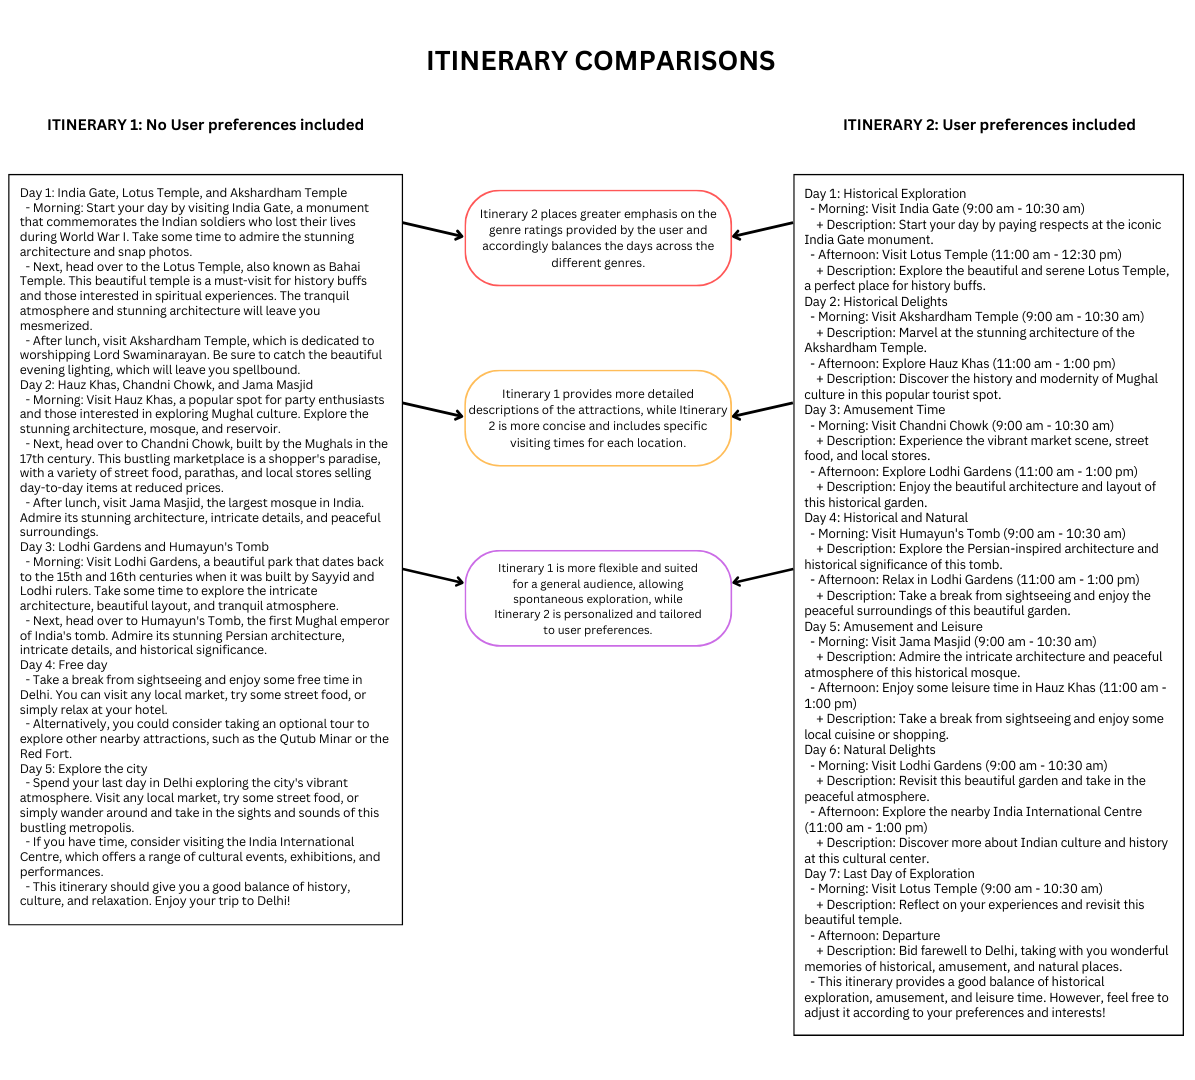
\includegraphics[width=0.9\textwidth]{Itinerary comparison.png} % Adjust the width to fit better
    \caption{Comparison of Itineraries With and Without User Preferences Included}
    \label{fig:itinerary_comparison}
\end{figure}

\newpage
.
\newpage

\subsection{Comparison of the Itineraries}

In Figure \ref{fig:itinerary_comparison}, a detailed comparison between two itineraries is presented: one that does not take user preferences into account (Itinerary 1) and another that does (Itinerary 2). There are three salient differences that can be observed between the two itineraries:

\begin{itemize}
\item \textbf{Genre Emphasis:} Itinerary 2 places greater emphasis on the genre ratings provided by the user and accordingly balances the days across the different genres.

\item \textbf{Detail Level:} Itinerary 1 provides more detailed descriptions of the attractions, while Itinerary 2 is more concise and includes specific visiting times for each location.

\item \textbf{Flexibility vs. Personalization:} Itinerary 1 is more flexible and suited for a general audience, allowing spontaneous exploration, while Itinerary 2 is personalized and tailored to user preferences.
\end{itemize}

Keeping these differences in mind, we sought to find which itinerary is more beneficial for our use case. On asking interview participants, 75\% chose the itinerary that considered user preferences and admired the level of personalization that comes with it. Some participants were even told to go beyond the selected four features: historical, natural, amusement, and cultural, and add several more valuable features.
\newpage

% \begin{acks}
% To Robert, for the bagels and explaining CMYK and color spaces.
% \end{acks}
% %%
% %% The next two lines define the bibliography style to be used, and
% %% the bibliography file.
% \bibliographystyle{ACM-Reference-Format}
% \bibliography{sample-base}


% %%
% %% If your work has an appendix, this is the place to put it.
% \appendix

% \section{Research Methods}

% \subsection{Part One}

% Lorem ipsum dolor sit amet, consectetur adipiscing elit. Morbi
% malesuada, quam in pulvinar varius, metus nunc fermentum urna, id
% sollicitudin purus odio sit amet enim. Aliquam ullamcorper eu ipsum
% vel mollis. Curabitur quis dictum nisl. Phasellus vel semper risus, et
% lacinia dolor. Integer ultricies commodo sem nec semper.

% \subsection{Part Two}

% Etiam commodo feugiat nisl pulvinar pellentesque. Etiam auctor sodales
% ligula, non varius nibh pulvinar semper. Suspendisse nec lectus non
% ipsum convallis congue hendrerit vitae sapien. Donec at laoreet
% eros. Vivamus non purus placerat, scelerisque diam eu, cursus
% ante. Etiam aliquam tortor auctor efficitur mattis.

\end{document}
\endinput
%%
%% End of file `sample-sigconf-authordraft.tex'.
